\documentclass[journal,12pt,twocolumn]{IEEEtran}
%
\usepackage{setspace}
\usepackage{gensymb}
%\doublespacing
\singlespacing

%\usepackage{graphicx}
%\usepackage{amssymb}
%\usepackage{relsize}
\usepackage[cmex10]{amsmath}
%\usepackage{amsthm}
%\interdisplaylinepenalty=2500
%\savesymbol{iint}
%\usepackage{txfonts}
%\restoresymbol{TXF}{iint}
%\usepackage{wasysym}
\usepackage{amsthm}
%\usepackage{iithtlc}
\usepackage{mathrsfs}
\usepackage{txfonts}
\usepackage{stfloats}
\usepackage{bm}
\usepackage{cite}
\usepackage{cases}
\usepackage{subfig}
%\usepackage{xtab}
\usepackage{longtable}
\usepackage{multirow}
%\usepackage{algorithm}
%\usepackage{algpseudocode}
\usepackage{enumitem}
\usepackage{mathtools}
\usepackage{steinmetz}
\usepackage{tikz}
\usepackage{circuitikz}
\usepackage{verbatim}
\usepackage{tfrupee}
\usepackage[breaklinks=true]{hyperref}
%\usepackage{stmaryrd}
\usepackage{tkz-euclide} % loads  TikZ and tkz-base
%\usetkzobj{all}
\usetikzlibrary{calc,math,backgrounds}
\usepackage{caption}
\usepackage{listings}
    \usepackage{color}                          %%
    \usepackage{array}                          %%
    \usepackage{longtable}                      %%
    \usepackage{calc}                           %%
    \usepackage{multirow}                       %%
    \usepackage{hhline}                         %%
    \usepackage{ifthen}                         %%
  %optionally (for landscape tables embedded in another document): %%
    \usepackage{lscape}     
\usepackage{multicol}
\usepackage{chngcntr}
%\usepackage{enumerate}
%\usepackage{wasysym}
%\newcounter{MYtempeqncnt}
\DeclareMathOperator*{\Res}{Res}
%\renewcommand{\baselinestretch}{2}
\renewcommand\thesection{\arabic{section}}
\renewcommand\thesubsection{\thesection.\arabic{subsection}}
\renewcommand\thesubsubsection{\thesubsection.\arabic{subsubsection}}
\renewcommand\thesectiondis{\arabic{section}}
\renewcommand\thesubsectiondis{\thesectiondis.\arabic{subsection}}
\renewcommand\thesubsubsectiondis{\thesubsectiondis.\arabic{subsubsection}}
% correct bad hyphenation here
\hyphenation{op-tical net-works semi-conduc-tor}
\def\inputGnumericTable{}                                 %%
\lstset{
%language=C,
frame=single, 
breaklines=true,
columns=fullflexible
}
%\lstset{
%language=tex,
%frame=single, 
%breaklines=true
%}
\begin{document}
%
\newtheorem{theorem}{Theorem}[section]
\newtheorem{problem}{Problem}
\newtheorem{proposition}{Proposition}[section]
\newtheorem{lemma}{Lemma}[section]
\newtheorem{corollary}[theorem]{Corollary}
\newtheorem{example}{Example}[section]
\newtheorem{definition}[problem]{Definition}
%\newtheorem{thm}{Theorem}[section] 
%\newtheorem{defn}[thm]{Definition}
%\newtheorem{algorithm}{Algorithm}[section]
%\newtheorem{cor}{Corollary}
\newcommand{\BEQA}{\begin{eqnarray}}
\newcommand{\EEQA}{\end{eqnarray}}
\newcommand{\define}{\stackrel{\triangle}{=}}
\bibliographystyle{IEEEtran}
%\bibliographystyle{ieeetr}
\providecommand{\mbf}{\mathbf}
\providecommand{\pr}[1]{\ensuremath{\Pr\left(#1\right)}}
\providecommand{\qfunc}[1]{\ensuremath{Q\left(#1\right)}}
\providecommand{\sbrak}[1]{\ensuremath{{}\left[#1\right]}}
\providecommand{\lsbrak}[1]{\ensuremath{{}\left[#1\right.}}
\providecommand{\rsbrak}[1]{\ensuremath{{}\left.#1\right]}}
\providecommand{\brak}[1]{\ensuremath{\left(#1\right)}}
\providecommand{\lbrak}[1]{\ensuremath{\left(#1\right.}}
\providecommand{\rbrak}[1]{\ensuremath{\left.#1\right)}}
\providecommand{\cbrak}[1]{\ensuremath{\left\{#1\right\}}}
\providecommand{\lcbrak}[1]{\ensuremath{\left\{#1\right.}}
\providecommand{\rcbrak}[1]{\ensuremath{\left.#1\right\}}}
\theoremstyle{remark}
\newtheorem{rem}{Remark}
\newcommand{\sgn}{\mathop{\mathrm{sgn}}}
\providecommand{\abs}[1]{\left\vert#1\right\vert}
\providecommand{\res}[1]{\Res\displaylimits_{#1}} 
\providecommand{\norm}[1]{\left\lVert#1\right\rVert}
%\providecommand{\norm}[1]{\lVert#1\rVert}
\providecommand{\mtx}[1]{\mathbf{#1}}
\providecommand{\mean}[1]{E\left[ #1 \right]}
\providecommand{\fourier}{\overset{\mathcal{F}}{ \rightleftharpoons}}
%\providecommand{\hilbert}{\overset{\mathcal{H}}{ \rightleftharpoons}}
\providecommand{\system}{\overset{\mathcal{H}}{ \longleftrightarrow}}
	%\newcommand{\solution}[2]{\textbf{Solution:}{#1}}
\newcommand{\solution}{\noindent \textbf{Solution: }}
\newcommand{\cosec}{\,\text{cosec}\,}
\providecommand{\dec}[2]{\ensuremath{\overset{#1}{\underset{#2}{\gtrless}}}}
\newcommand{\myvec}[1]{\ensuremath{\begin{pmatrix}#1\end{pmatrix}}}
\newcommand{\mydet}[1]{\ensuremath{\begin{vmatrix}#1\end{vmatrix}}}
%\numberwithin{equation}{section}
\numberwithin{equation}{subsection}
%\numberwithin{problem}{section}
%\numberwithin{definition}{section}
\makeatletter
\@addtoreset{figure}{problem}
\makeatother
\let\StandardTheFigure\thefigure
\let\vec\mathbf
%\renewcommand{\thefigure}{\theproblem.\arabic{figure}}
\renewcommand{\thefigure}{\theproblem}
%\setlist[enumerate,1]{before=\renewcommand\theequation{\theenumi.\arabic{equation}}
%\counterwithin{equation}{enumi}
%\renewcommand{\theequation}{\arabic{subsection}.\arabic{equation}}
\def\putbox#1#2#3{\makebox[0in][l]{\makebox[#1][l]{}\raisebox{\baselineskip}[0in][0in]{\raisebox{#2}[0in][0in]{#3}}}}
     \def\rightbox#1{\makebox[0in][r]{#1}}
     \def\centbox#1{\makebox[0in]{#1}}
     \def\topbox#1{\raisebox{-\baselineskip}[0in][0in]{#1}}
     \def\midbox#1{\raisebox{-0.5\baselineskip}[0in][0in]{#1}}
\vspace{3cm}
\title{Matrix Theory(EE5609) Assignment 4}
\author{Anshum Agrawal \\ Roll No- AI20MTECH11006}
%
\maketitle
\newpage
%\tableofcontents
\bigskip
\renewcommand{\thefigure}{\theenumi}
\renewcommand{\thetable}{\theenumi}
%\renewcommand{\theequation}{\theenumi}
%\begin{abstract}
%%\boldmath
\begin{abstract}
  This Assignment proves the property of a given triangle 
\end{abstract}
%
Download latex-tikz codes from 
%
\begin{lstlisting}
https://github.com/anshum0302/EE5609/blob/master/assignment4/assign4.tex
\end{lstlisting}
%
\section{\textbf{PROBLEM STATEMENT}}
$\triangle{ABC}$ is an isosceles triangle in which AB = AC. Side BA is produced to D such that AD = AB. Show that $\angle{BCD}$ is a right angle.

\section{\textbf{Solution}}
\renewcommand{\thefigure}{\arabic{figure}}
\begin{figure}[!h]
  \centering
    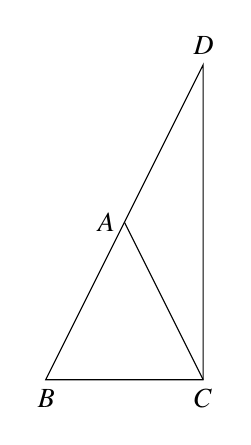
\begin{tikzpicture}
      \coordinate (A) at (1,2) {};
      \coordinate (B) at (0,0) {};
      \coordinate (C) at (2,0) {};
      \coordinate (D) at (2,4) {};
      \draw (B)node[below]{$B$}--(C)node[below]{$C$}--(D)node[above]{$D$}--cycle;
      \draw (A)node[left]{$A$}--(C);
    \end{tikzpicture}
  \caption{}
  \label{myfig}
\end{figure}
We are given that AB = AC. So
\begin{align}
  \norm{\vec{A-B}} = \norm{\vec{A-C}} \label{eq1}
\end{align}
Also BA is produced to D such that AB = AD. Therefore we have
\begin{align}
  \vec{A-B} = \vec{D-A} \label{eq2}
\end{align}
Taking dot product of vectors $\vec{(B-C)}$ and $\vec{(D-C)}$ we get
\begin{align*}
  &\vec{(B-C)}^T\vec{(D-C)}\\
  &= \vec{(B-A+A-C)}^T\vec{(D-A+A-C)}\\
  &= \vec{((B-A)+(A-C))}^T\vec{((D-A)+(A-C))}
\end{align*}
using \eqref{eq2} we get
\begin{align*}
  &\vec{(B-C)}^T.\vec{(D-C)} \\
  &= \vec{((B-A)+(A-C))}^T\vec{((D-A)+(A-C))}\\
  &= \vec{((B-A)+(A-C))}^T\vec{((A-B)+(A-C))}\\
  &= \vec{(-(A-B)+(A-C))}^T\vec{((A-B)+(A-C))}\\
  \begin{split}
    &= -\norm{\vec{A-B}}^2-\vec{(A-B)}^T\vec{(A-C)}\\
    &\qquad +\vec{(A-C)}^T\vec{(A-B)}+\norm{\vec{A-C}}^2
  \end{split}
\end{align*}
now $\vec{(A-B)}^T\vec{(A-C)}$ and $\vec{(A-C)}^T\vec{(A-B)}$ are both dot product of vectors $\vec{(A-B)}$ and $\vec{(A-C)}$,therefore
\begin{align*}
  \begin{split}
    &\vec{(B-C)}^T.\vec{(D-C)} \\
    &= -\norm{\vec{A-B}}^2-\vec{(A-B)}^T\vec{(A-C)}\\
                                &\qquad +\vec{(A-C)}^T\vec{(A-B)}+\norm{\vec{A-C}}^2
  \end{split}\\
  &= -\norm{\vec{A-B}}^2+\norm{\vec{A-C}}^2
\end{align*}
using \eqref{eq1} we get
\begin{align}
  \vec{(B-C)}^T.\vec{(D-C)} &= -\norm{\vec{A-B}}^2+\norm{\vec{A-C}}^2 = 0
\end{align}
since $\vec{(B-C)}^T.\vec{(D-C)}$ = 0,therefore BC $\perp$ CD and $\angle{BCD}$ is a right angle.
\end{document}
